\Askhsh{22051}{2}
\begin{ylh}{1}
    \item 3.4 Η Υπερβολή.
\end{ylh}
\begin{center}
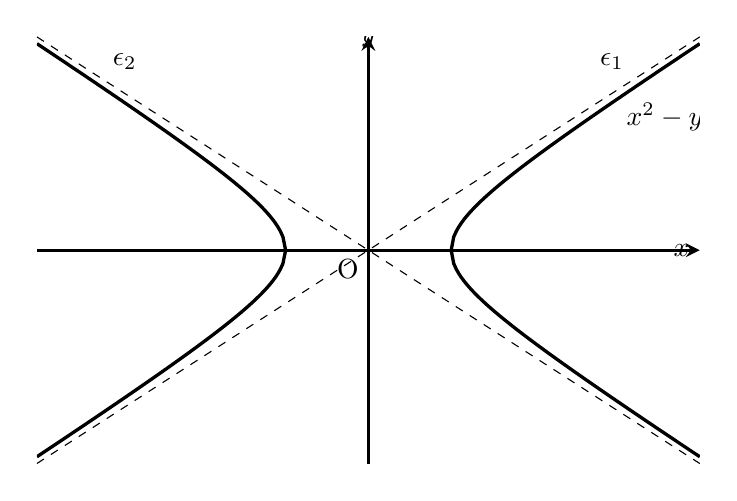
\begin{tikzpicture}
\begin{axis}[
    axis lines = middle,
    xmin = -4, xmax = 4,
    ymin = -4, ymax = 4,
    width = 10cm, height = 7cm,
    axis line style={very thick},
    % Hide default ticks and labels, as they are not shown in the image beyond the axis labels
    xtick style={draw=none},
    ytick style={draw=none},
    xticklabels={},
    yticklabels={},
]
    % Hyperbola x^2 - y^2 = 1
    \addplot[very thick, black, domain=1:4, samples=100] {sqrt(x^2 - 1)};
    \addplot[very thick, black, domain=1:4, samples=100] {-sqrt(x^2 - 1)};
    \addplot[very thick, black, domain=-4:-1, samples=100] {sqrt(x^2 - 1)};
    \addplot[very thick, black, domain=-4:-1, samples=100] {-sqrt(x^2 - 1)};

    % Asymptotes y = x and y = -x
    \addplot[dashed, black, domain=-4:4] {x}; % Asymptote epsilon_1
    \addplot[dashed, black, domain=-4:4] {-x}; % Asymptote epsilon_2

    % Labels for axes and origin
    \node[right, xshift=2pt] at (axis cs:3.5,0) {$x$}; % X-axis label
    \node[above, yshift=2pt] at (axis cs:0,3.5) {$y$}; % Y-axis label
    \node[below left] at (axis cs:0,0) {O}; % Origin label

    % Asymptote labels epsilon_1 and epsilon_2
    \node[above left] at (axis cs:3.2,3.2) {$\epsilon_1$};
    \node[above right] at (axis cs:-3.2,3.2) {$\epsilon_2$};

    % Hyperbola equation label
    \node[right] at (axis cs:3,2.5) {$x^2 - y^2 = 1$};
\end{axis}
\end{tikzpicture}
\end{center}
Δίνεται η υπερβολή $x^2 - y^2 = 1$. Να αποδείξετε για τις ασύμπτωτες ευθείες $\epsilon_1$ και $\epsilon_2$ της υπερβολής ότι:
\begin{alist}
\item Συμπίπτουν με την διχοτόμο του $1^{\text{ου}}$ και $3^{\text{ου}}$ τεταρτημορίου και την διχοτόμο του $2^{\text{ου}}$ και $4^{\text{ου}}$ τεταρτημορίου, αντίστοιχα. \monades{13}
\item Είναι ευθείες κάθετες μεταξύ τους. \monades{12}
\end{alist}